\lab{Inverse Problems}{Inverse Problems}
\label{lab:inverse_problems}

% \objective{ }
An important concept in mathematics is the idea of a well posed problem. The concept initially came from Jacques Hadamard. A mathematical problem is \textit{well posed} if 
\begin{enumerate}
	\item a solution exists, 
	\item that solution is unique, and 
	\item the solution is continuously dependent on the data in the problem. \label{inverse_problems:continuous_dependence}
\end{enumerate}
A problem that is not well posed is \textit{ill posed}. Notice that a problem may be well posed, and yet still possess the property that small changes in the data result in larger changes in the solution; in this case the problem is said to be \text{ill conditioned}, and has a large \text{condition number}.

Note that for a physical phenomena, a well posed mathematical model would seem to be a necessary requirement! However, there are important examples of mathematical problems that are ill posed. For example, consider the process of differentiation. Given a function $u$ together with its derivative $u'$, let $\tilde{u}(t) = u(t) +  \epsilon \sin(\epsilon^{-2}t)$ for some small $\epsilon > 0$. Then note that 
\begin{align*}
	\|u-\tilde{u}\|_{\infty} &= \epsilon,
\end{align*}
while
\begin{align*}
	\|u'-\tilde{u}'\|_{\infty} &= \epsilon^{-1}.
\end{align*}
Since a small change in the data leads to an arbitrarily large change in the output, differentiation is an ill posed problem. And we haven't even mentioned numerically approximating a derivative!

For an example of an ill posed problem from PDEs, consider the backwards heat equation with zero Dirichlet conditions: 
\begin{align}
\begin{split}
	&{} u_t = -u_{xx}, \quad (x,t) \in (0,L)\times (0,\infty),\\
	&{} u(0,t) = u(L,t) = 0, \quad t \in (0,\infty),\\
	&{} u(x,0) = f(x), \quad x \in (0,L).
\end{split}
\end{align}
For the initial data $f(x)$ the unique\footnote{See \textit{Partial Differential Equations} by Lawrence C. Evans, chapter 2.3, for a proof of uniqueness.} solution is $u(x,t) = 0.$ 
Given the initial data $f(x) = \frac{1}{n}\sin ( \frac{n \pi x}{L})$, one can check that there is a unique solution $u(x,t) = \frac{1}{n}\sin ( \frac{n \pi x}{L})\exp ( (\frac{n \pi }{L})^2 t)$. 
Thus, on a finite interval $[0,T]$, as $n \to \infty$ we see that a small difference in the initial data results in an arbitrarily large difference in the solution.



\section*{Inverse Problems}
As implied by the name, inverse problems come in pairs. For example, differentiation and integration are inverse problems. The easier problem (in this case integration) is often called the direct problem. The direct problem is usually studied first historically.

Given a physical system, together with initial data (the "cause"), the direct problem will usually predict the future state of the physical system (the "effect"); see Figure \ref{fig:cause_and_effect}.  Inverse problems often turn this on its head - given the current state of a physical system (at say time $T$), what was the physical state at time $t = 0$?  

Alternatively, suppose we measure the current state of the system, and we then measure the state at some future time. An important inverse problem is to determine an appropriate mathematical model that can describe the evolution of the system.



\begin{figure}
\centering
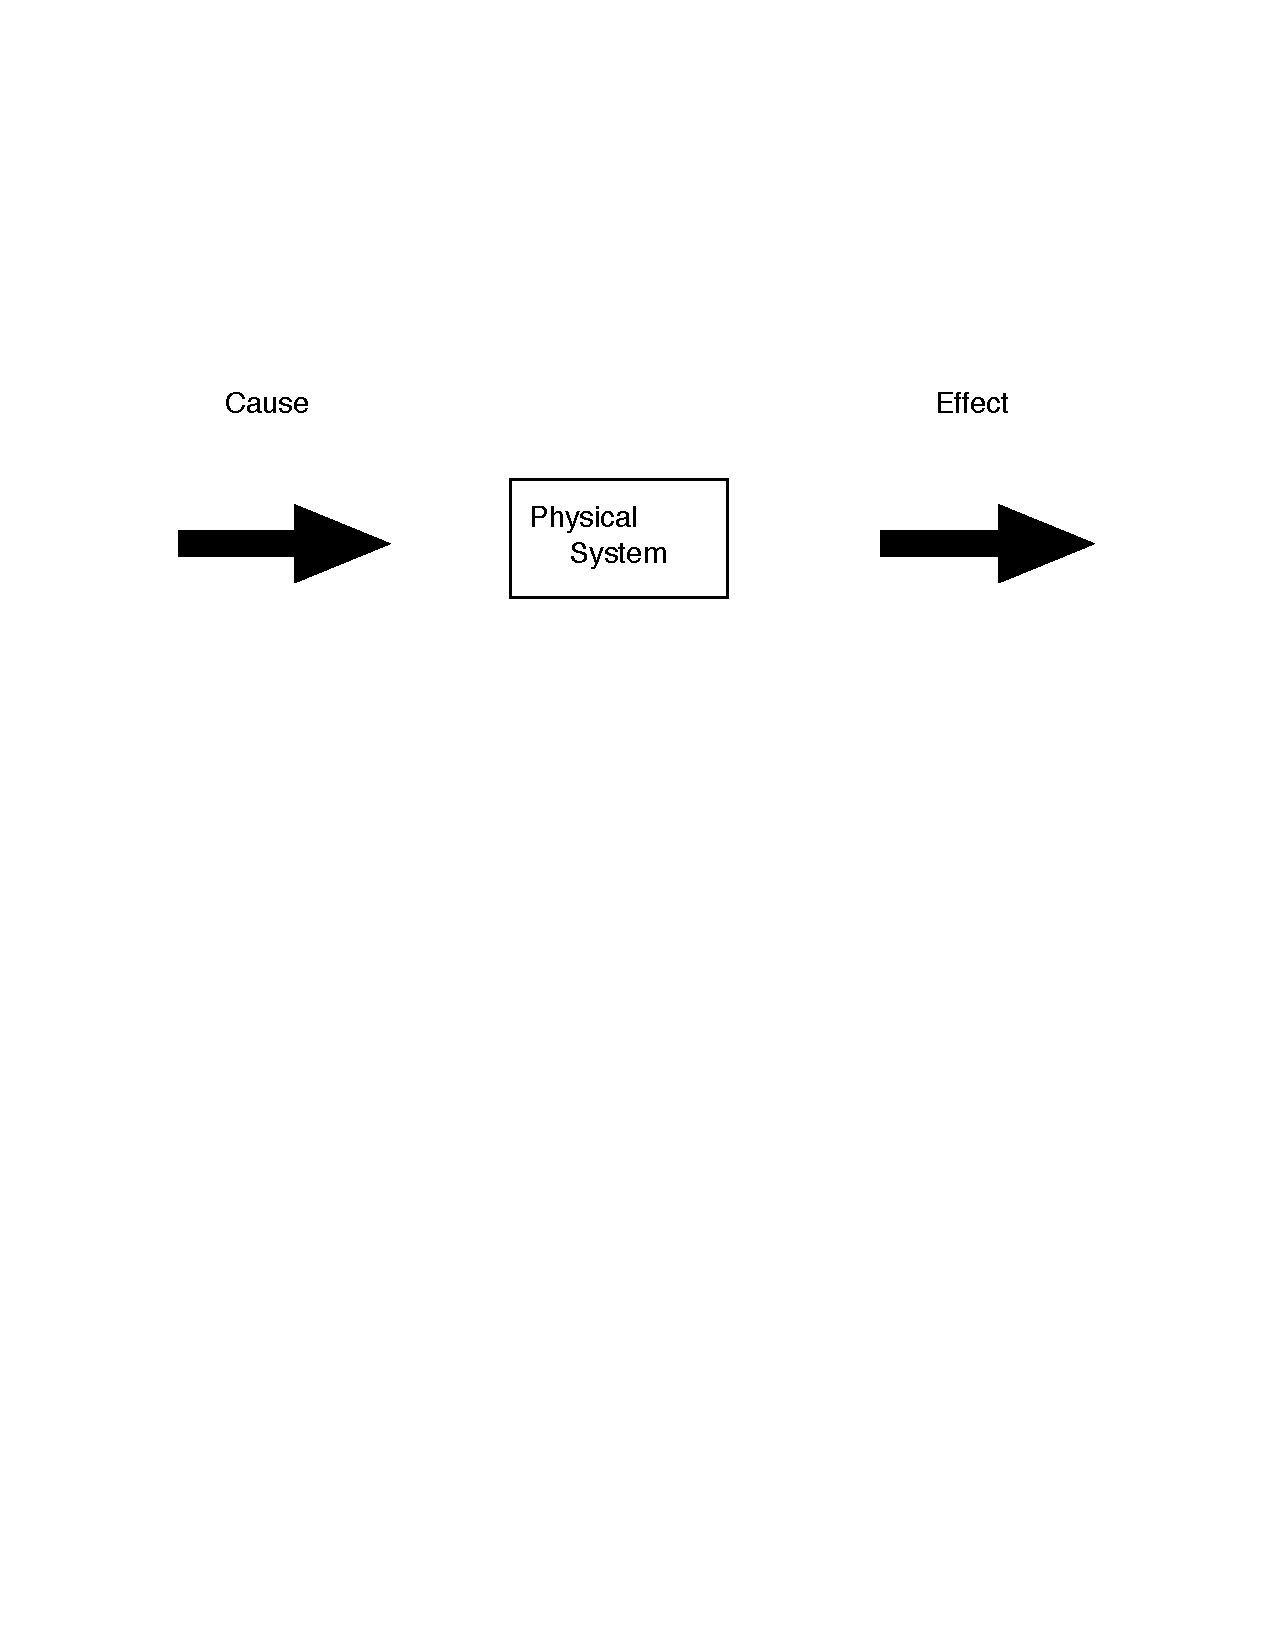
\includegraphics[width=\textwidth]{cause_and_effect.pdf}
\caption{Cause and effect within a given physical system.}
\label{fig:cause_and_effect}
\end{figure}

\section*{Another look at heat flow through a rod}
Consider the ordinary differential equation, together with natural boundary conditions at the ends of the interval: 
\begin{align}
\begin{cases}
	-(au')' = f, & x \in (0,1),\\
	a(0)u'(0) = c_0, & a(1)u'(1) = c_1.
\end{cases} \label{inverse_problems:heat_flow}
\end{align}
This BVP can, for example, be used to describe the flow of heat through a rod. The boundary conditions would correspond the specifying the heat flux through the ends of the rod. $f(x)$ would then represent external heat sources along the rod, and $a(x)$ the density of the road at each point. 

Typically, the density $a(x)$ would be specified, along with any heat sources $f(x)$, and the (direct) problem is to solve for the steady-state heat distribution $u(x)$. Here we shake things up a bit: suppose the heat sources $f$ are given, and we can measure the heat distribution $u(x)$. Can we find the density of the rod? This is an example of a \textit{parameter estimation problem}.

Let us consider a numerical method for solving \eqref{inverse_problems:heat_flow} for the density $a(x)$.
%  where 
% $c_0 = 3/8,$ $c_1 = 5/4$, $u(x) = x^2 + x/2 + 5/16$, and 
% \begin{align*}
% 	f &= \begin{cases}
% 		-6x^2 + 6x - 5/2 & x \in [0,1/2],\\
% 		-1 & x \in (1/2,1].
% 	\end{cases}
% \end{align*}
Subdivide $[0,1]$ into $N$ equal subintervals, and let $x_j = jh$, $j = 0, \ldots,N$, where $h = 1/N$.
Let $\phi_j(x)$ be the tent functions (used earlier in the finite element lab), given by 
\begin{align*}
	\phi_j(x) = \begin{cases}
(x - x_{j-1})/h  &  x \in [x_{j-1},x_j],\\
 (x_{j+1} - x)/h  &  x \in [x_{j},x_{j+1}],\\
0 & \text{ otherwise.}
\end{cases}
\end{align*}
We look for an approximation $a^h(x)$ of the form 
\begin{align}
	a^h &= \sum_{j=0}^N \alpha_j \phi_j. \label{inverse_problems:approximate}
\end{align}

Integrating \eqref{inverse_problems:heat_flow} from $0$ to $x$, we obtain
\begin{align}
\begin{split}
&{} \int_0^x -(au')'\, ds = \int_0^x f(s)\, ds,\\
&{} -[a(x)u'(x) - c_0] = \int_0^x f(s)\, ds,\\
&{} u'(x) = \frac{c_0 - \int_0^x f(s)\, ds}{a(x)}.
\end{split}
\end{align}
Thus for each $x_j$
\begin{align*}
	u'(x_j) &= \frac{c_0 - \int_0^{x_j} f(s)\, ds}{a(x_j)},\\
	&= \frac{c_0 - \int_0^{x_j} f(s)\, ds}{\alpha_j}.
\end{align*}
The coefficients $\alpha_j$ in \eqref{inverse_problems:approximate} can now be approximated by minimizing 
\begin{align*}
	\sum_{j=0}^N \left( \frac{c_0 - \int_0^{x_j} f(s)\, ds}{\alpha_j} - u'(x_j)  \right)^2.
\end{align*}

For $c_0 = 3/8,$ $c_1 = 5/4$, $u(x) = x^2 + x/2 + 5/16$, and 
\begin{align*}
	f &= \begin{cases}
		-6x^2 + 3x - 1 & x \leq 1/2,\\
		-1 & 1/2 < x \leq 1,
	\end{cases}
\end{align*}
we partially implement this method with the following code:


\begin{lstlisting}
import numpy as np
from scipy.optimize import minimize
import matplotlib.pyplot as plt

def f(x):
	out = -np.ones(x.shape)
	m = np.where(x<.5)
	out[m] = -6*x[m]**2. + 3.*x[m] - 1.
	return out

def u(x):
	return (x+1./4)**2. + 1./4

def integral_of_f(x):
	# out =  \int_0^x f(s) ds
	return out

def derivative_of_u(x):
	# out = u'(x)
	return out

x = np.linspace(0,1,11)
F, u_p = integral_of_f(x), derivative_of_u(x)

def sum_of_squares(alpha):
	pass

guess = (1./4)*(3-x)
sol = minimize(sum_of_squares,guess)

plt.plot(x,sol.x,'-ob',linewidth=2)
plt.show()
\end{lstlisting}


\begin{figure}
\centering
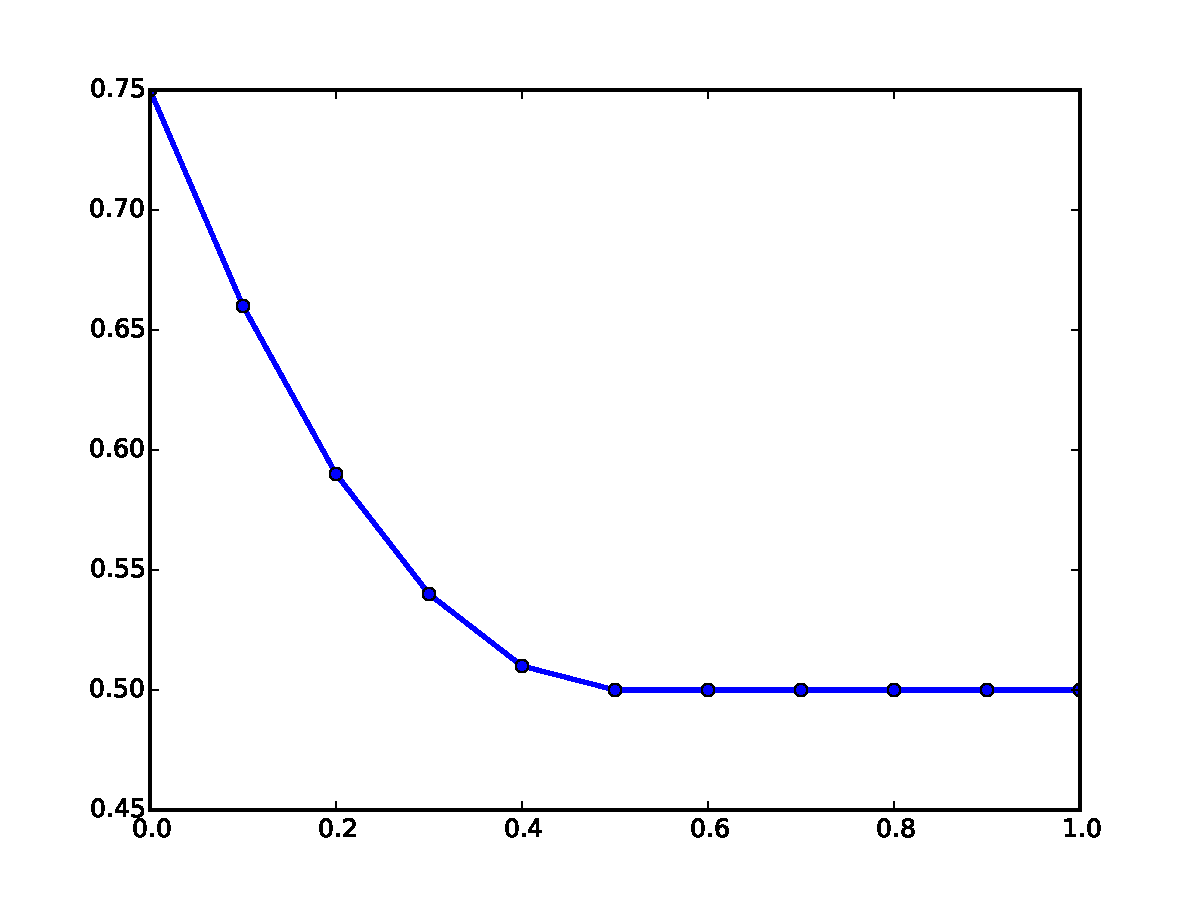
\includegraphics[width=\textwidth]{density_a.pdf}
\caption{The solution $a(x)$ computed by the example code.}
\label{fig:inverse_problems:num1}
\end{figure}


\begin{problem}
	Finish the previous code block to solve \eqref{inverse_problems:heat_flow} for $a(x)$.
	Produce the plot shown in Figure \ref{fig:inverse_problems:num1}.
\end{problem}

\begin{problem}
	Find the density function $a(x)$ satisfying 
	\begin{align}
	\begin{cases}
		-(au')' = -1, & x \in (0,1),\\
		a(0)u'(0) = 1, & a(1)u'(1) = 2.
	\end{cases} \label{inverse_problems:ill_posed}
	\end{align}
	where $u(x) = x + 1 + \epsilon \sin(\epsilon^{-2}x)$.  Using several values of $\epsilon  > 0.66049142$, plot the corresponding density $a(x)$ to demonstrate that the problem is ill-posed.
\end{problem}

\begin{figure}
\centering
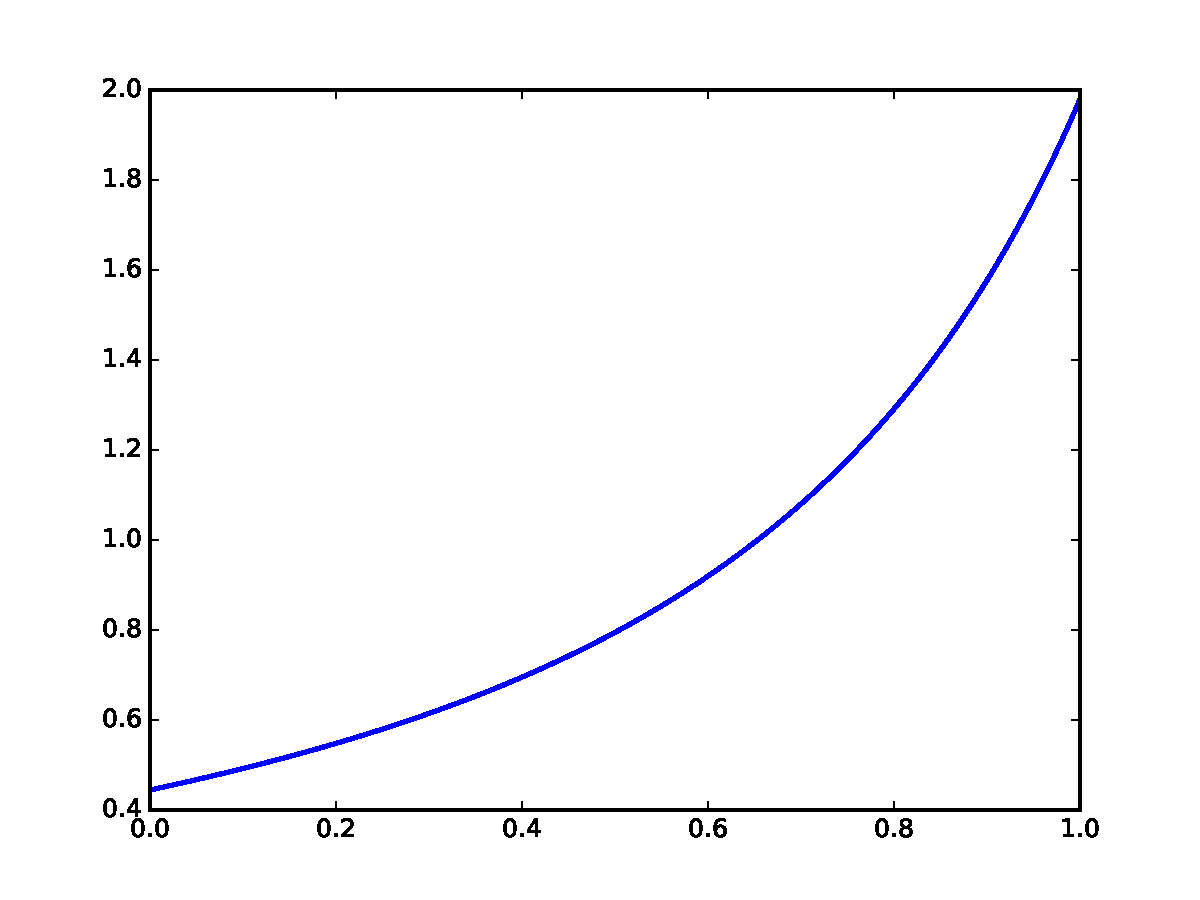
\includegraphics[width=\textwidth]{ill_posed_density_a.pdf}
\caption{The density function $a(x)$ satisfying \eqref{inverse_problems:ill_posed} for $\epsilon = .8$.}
\label{fig:inverse_problems:exercise1}
\end{figure}


% \begin{align*}
% 	a(x) &=
% 	\begin{cases}
% 		x^2 - x + 3/4 & x \leq 1/2,\\
% 		\frac{1}{2} & 1/2 < x \leq 1.
% 	\end{cases}
% \end{align*}




% \begin{align*}
% 	au'(x) &=
% 	\begin{cases}
% 		(x^2 - x + 3/4)(2x - 1) & x \leq 1/2,\\
% 		\frac{1}{2}(2x - 1) & 1/2 < x \leq 1.
% 	\end{cases}
% \end{align*}

% \begin{align*}
% 	au'(x) &=
% 	\begin{cases}
% 		(x^2 - x + 3/4)(2x - 1) & x \leq 1/2,\\
% 		\frac{1}{2}(2x - 1) & 1/2 < x \leq 1.
% 	\end{cases}\\
% 	(au'(x))' &= 
% 	\begin{cases}
% 		6x^2 - 6x + 5/2 & x \leq 1/2,\\
% 		1 & 1/2 < x \leq 1.
% 	\end{cases}\\
% 	&= -f
% \end{align*}


% \begin{align*}
% 	u(x) &= (x+1/4)^2 + 1/4 = x^2 + x/2 + 5/16,\\
% 	f &= \begin{cases}
% 		-6x^2 + 6x - 5/2 & x \leq 1/2,\\
% 		-1 & 1/2 < x \leq 1.
% 	\end{cases}\\
% 	a(x) &=
% 	\begin{cases}
% 		x^2 - x + 3/4 & x \leq 1/2,\\
% 		\frac{1}{2} & 1/2 < x \leq 1.
% 	\end{cases}
% \end{align*}

% \begin{align}
% 	
% \end{align}
 
% \textit{}
% \footnote{}
% \label{inverse_problems:}
% \eqref{inverse_problems:}

% \begin{lstlisting}
% \end{lstlisting}

% \begin{figure}
% \centering
% \includegraphics[width=\textwidth]{.pdf}
% \caption{}
% \label{fig:inverse_problems}
% \end{figure}





